\documentclass[conference]{IEEEtran}
\IEEEoverridecommandlockouts
% The preceding line is only needed to identify funding in the first footnote. If that is unneeded, please comment it out.
\usepackage{cite}
\usepackage{amsmath,amssymb,amsfonts}
\usepackage{algorithmic}
\usepackage{graphicx}
\usepackage{textcomp}
\usepackage[utf8]{inputenc}
\def\BibTeX{{\rm B\kern-.05em{\sc i\kern-.025em b}\kern-.08em
    T\kern-.1667em\lower.7ex\hbox{E}\kern-.125emX}}
\begin{document}

\title{Reporte de prácticas\\
\thanks{Identify applicable funding agency here. If none, delete this.}
}

\author{\IEEEauthorblockN{1\textsuperscript{st} René Muñoz Sánchez}
\IEEEauthorblockA{\textit{Sistemas Programables} \\
\textit{Instituto Tecnológico de Toluca}\\
Metepec, México \\
r@renems.com}

% \and
% \IEEEauthorblockN{2\textsuperscript{nd} Given Name Surname}
% \IEEEauthorblockA{\textit{dept. name of organization (of Aff.)} \\
% \textit{name of organization (of Aff.)}\\
% City, Country \\
% email address}

% \and
% \IEEEauthorblockN{2\textsuperscript{nd} Given Name Surname}
% \IEEEauthorblockA{\textit{dept. name of organization (of Aff.)} \\
% \textit{name of organization (of Aff.)}\\
% City, Country \\
% email address}

}

\maketitle

\begin{abstract}
Este documento plasma el proceso de desarrollo de un circuito utilizando un sensor de movimiento PIR y un fotorresistor LDR para la detección de movimiento, nivel de iluminación del ambiente y color.
\end{abstract}

\begin{IEEEkeywords}
arduino, sensores, sistemas, programables
\end{IEEEkeywords}

\section{Introduccion}
En el siguiente documento se plasma el proceso utilizado para desarrollar un programa en un microcontrolador Arduino Mega 2560, con el fin de mostrar los valores resultantes de utilizar el sensor de movimiento PIR y una fotorresistencia LDR para detectar los lumenes encontrados en el ambiente. Los valores de los parámetros utilizados para obtener dichos resultados son mostrados al usuario a través de una pantalla TFT Shield (una pantalla LCD externa conectada directamente al Arduino), además de en una hyperterminal, una interfaz de usuario creada utilizando el lenguaje de programación Java, que grafica en tiempo real los valores resultantes de acuerdo con los cambios encontrados.

Además, los valores de los parámetros pueden ser modificados desde la pantalla a través de un teclado matricial gráfico, siendo estos guardados en la memoria interna del microcontrolador (EEPROM), modificando los cálculos posteriores.

\section{Objetivos}

\begin{itemize}
  \item Utilizando un sensor de movimiento PIR, detectar el movimiento de un cuerpo.
  \item Utilizando una fotorresistencia LDR, detectar los lúmenes encontrados en el ambiente.
  \item Utilizando una fotorresistencia LDR y un diodo emisor de luz (LED) de color blanco conectado a una resistencia de 10K ohms, detectar los colores blanco, negro, azul, rojo y amarillo.
  \item Calibrar los parámetros necesarios a través de la pantalla LCD táctil, y guardar los cambios en la memoria interna del microcontrolador Arduino (la memoria EEPROM).
  \item Mostrar los valores de los sensores en la pantalla LCD.
  \item Graficar en tiempo real a través de una hyperterminal los resultados de la detección de lúmenes, color y movimiento.
\end{itemize}

\section{Marco teorico}

Sensor de movimiento: un sensor infrarrojo pasivo PIR (Passive infrared sensor, por sus siglas en ingles), mide la luz infrarroja que sale de un objeto en su área visible. Más precisamente, estos sensores pueden detectar cambios en sus campos de visión, como cuando la luz infrarroja ambiental se interrumpe o se altera de otra manera. [1] También llamados detectores de movimiento IR y sensores piroeléctricos, generalmente son bastante pequeños en tamaño, desde una pulgada o menos hasta alrededor de cuatro pulgadas para uso doméstico y comercial estándar. Los sensores PIR tienen vidas muy largas y no suelen ser costosos de producir, lo que los convierte en opciones valiosas y económicas para su uso en muchas industrias y aplicaciones. Los sensores PIR son lentes sensibles a la luz controlados por y montados en placas de circuito que permiten la calibración para temperaturas específicas, tamaños de objetos y ubicaciones o dirección de movimiento. [2]

Fotorresistencia: las fotorresistencias o fotoconductores (en ingles, Light Dependent Resistors LDR) se basan en la variacion de la resistencia electrica de un semiconductor al incidir en el radiacion optica (radiacion electromagnetica con longitud de onda entre 1 mm y 10 nm). Las fotorresistencias varían su resistencia según la iluminación. Para ello se metaliza el metal semiconductor, por ejemplo sulfuro de cadmio (CdS), en forma de película delgada sobre un soporte, por ejemplo vidrio, y se instala bajo cristal en un encapsulado. Las otras resistencias aprovechan el efecto fotoeléctrico interno. La enegía de los rayos luminosos liberan en el interior del semiconductor nuevas parejas de portadores de cargas (electrones y huecos). Cuando termina la iluminación, los electrones vuelven a su estado original recombinado (recombinación). La conductvidad de la fotorresistencia aumenta al aumentar la intesidad de iluminación, es decir, que se reduce la resistencia. Se distingue entre los valores característicos de resistencia de claridad R\textsubscript{h} y de resistencia de oscuridad R\textsubscript{d}. [3]

Para obtener el valor de los luxes es necesario obtener la representación digital del valor del voltaje analógico utilizando la función analogRead provista para Arduino. Posteriormente, la representación digital debe ser convertida en voltaje escalando el valor del convertidor analógico a digital al valor de referencia del voltaje. El valor máximo posible de lectura del ADC es 1023, mientras que el voltaje de referencia es de 5.0 V: $ \ voltajeResistor = \frac{analogRead(pinLDR)}{1023} * 5.0 $.
Posteriormente, el voltaje en la fotorresistencia debe ser determinado. Ya que los 5.0 V provistos son divididos entre el resistor de 10K ohms y la fotorresistencia, es necesario substraer el voltaje de la resistencia de los 5 V: $ \ voltajeLDR =  5.0 - voltajeResistor$.
Finalmente, la resistencia del LDr debe ser calculada basado en el voltaje. El valor de 10,000 representa la resistencia conectada de la siguiente manera: $ \ resistenciaLDR = \frac{voltajeLDR}{voltajeResistor} * 10000 $.
Una vez obtenida la resistencia, la iluminación en luxes puede ser calculada de la siguiente manera: $ \ luxesLDR = luxEscalar * resistenciaLDR^{luxExponente} $. Vista de otra manera la ecuación de la iluminación en luxes resultante es: $ \ luxes = A * Resistencia^{B} $, donde A es la resistencia en la oscuridad (en ohms), Resistencia es el valor del resistor utilizado (por ejemplo, 10K ohms) y B es el valor de la resistencia a la luz (10 Lux) en K ohms.

Diodo emisor de luz: LED por sus siglas en inglés (light-emitting diode) es un diodo de unión p-n, fabricado casi siempre con un material semiconductor como el arseniuro de aluminio y galio (AlGaAs) o el arseniuro fosfuro de galio (GaAsP). Los LED emiten luz por emisión espontánea: la luz se emite como resultado de la recombinación de electrones con huecos. Cuando tienen polarización directa, los portadores minoritarios se inyectan a través de la unión p-n. Una vez atravesada la unión, esos portadores minoritarios se recombinan con portadores mayoritarios y desprenden energía en forma de luz. [4]

Arduino Mega 2560: El Arduino Mega 2560, es un microcontrolador basado en un microcontrolador ATmega2560 AVR. Cuenta con 70 pines digitales de entrada / salida (de los cuales 14 se pueden utilizar como salidas PWM y 16 se pueden utilizar como entradas analógicas), un resonador de 16 MHz, una conexión USB, un conector de alimentación, una programación en circuito (ICSP) y un botón de reinicio. [5]

Hyperterminal: Es un programa que puede usarse para conectarse a otras computadoras, sitios Telnet, BBS (boletin board systems), servicios en línea y computadoras host. Las conexiones se hacen usando un módem, un cable de módem nulo (utilizado para emular la comunicación de módem), una conexión de Ethernet o un cable USB. [6]

TFT Shield: Es una pantalla TFT de 2.8 pulgadas de 240x320 pixeles resistiva, lo que la hace capaz de detectar huellas dactilares en cualquier parte de la pantalla. Tiene una capacidad de hasta 262,000 tonos diferentes. [7]

Memoria EEPROM: EEPROM significa memoria de solo lectura programable borrable eléctricamente y es un tipo de memoria no volátil utilizada en computadoras y otros dispositivos electrónicos para almacenar cantidades relativamente pequeñas de datos pero que permiten borrar y reprogramar bytes individuales. Las EEPROM están organizadas como matrices de transistores de puerta flotante. Las EEPROM pueden programarse y borrarse en el circuito, mediante la aplicación de señales de programación especiales. Originalmente, las EEPROM se limitaban a operaciones de un solo byte que las hacían más lentas, pero las EEPROM modernas permiten operaciones de página de múltiples bytes. También tiene una vida limitada para borrado y reprogramación, alcanzando ahora un millón de operaciones en las EEPROM modernas. En una EEPROM que se reprograma frecuentemente mientras la computadora está en uso, la vida de la EEPROM es una consideración de diseño importante. [8]

\section{Desarrollo}

\subsection{Material utilizado}
\begin{itemize}
  \item 1 microcontrolador Arduino Mega 2560.
  \item 1 sensor de movimiento PIR.
  \item 1 fotorresistencia LDR.
  \item 1 diodo emisor de luz (LED) color blanco.
  \item 1 pantalla TFT Shield.
  \item 1 resistencia de 10K ohms.
  \item 1 resistencia de 330 ohms. 
  \item Cables conectores macho-macho.
\end{itemize}

\subsection{Programacion del microcontrolador}
\begin{figure}
  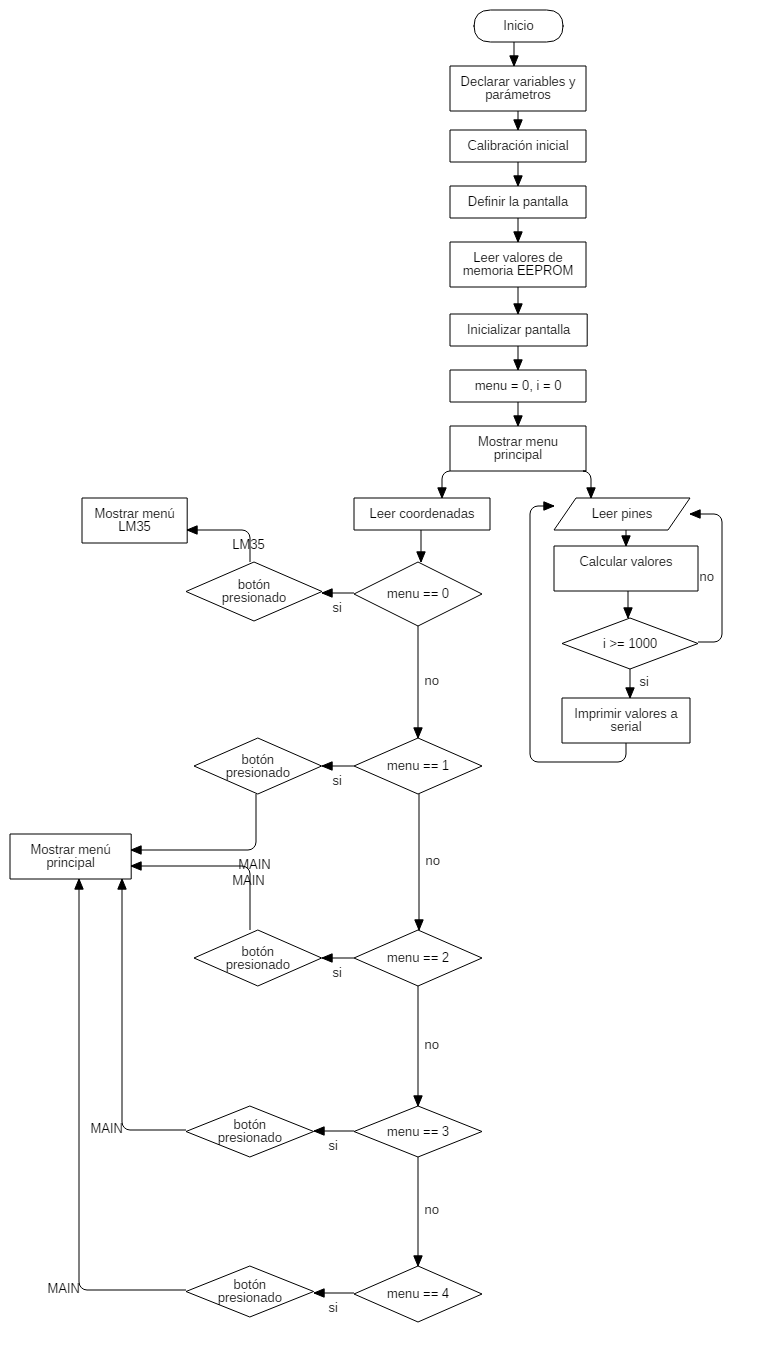
\includegraphics[width=\linewidth]{fig1_diagram_Arduino.png}
  \caption{Diagrama de flujo de la programacion del microcontrolador}
  \label{fig:flowDiagram1}
\end{figure}

Para realizar la programación del microcontrolador se toma en cuenta la estructura de todo programa en Arduino o sketch, que consta de dos métodos principales.

En primer lugar se tiene el método void setup(), en el que se declaran las instrucciones a realizarse al momento de ejecución del microcontrolador

En este método se realiza:
\begin{itemize}
  \item La configuración del puerto serial, con una tasa de baudios de 9600.
  \item La configuración de los pines necesarios de la pantalla y de los sensores.
  \item La lectura inicial de los valores de las variables de calibración de los sensores desde la memoria EEPROM del microcontrolador.
  \item Se establecen los parámetros iniciales de la configuración de la pantalla LCD, como son la rotación de la pantalla (en grados) y el color de fondo inicial.
  \item Se muestra el menú inicial.
\end{itemize}

A continuación, se tiene el método void loop(), que se ejecuta continuamente mientras está encendido el microcontrolador. Este método realiza dos tareas principales: leer las coordenadas en donde el usuario presiona la pantalla para realizar tareas correspondientes, y en segundo lugar se realizan las lecturas y los cálculos de todos los sensores. En seguida se detalla el procedimiento general:
\begin{enumerate}
  \item En primer lugar, se obtienen la lectura de las coordenadas presionadas por el usuario en la pantalla. Dependiendo del menú en el que se encuentre el mismo, se simula la acción de presionar botones con el fin de realizar diversas tareas, como son el moverse a un menú diferente o, en su caso, mostrar un teclado matricial para realizar la calibración de un parámetro de un sensor.
  \item En segundo lugar, se realizan las operaciones de cálculo de los valores requeridos. En el caso del sensor de movimiento PIR, se realiza la lectura de su pin digital correspondiente, pudiendo obtenerse dos valores (un 0 en el caso de que no se detecte movimiento, o 1 en caso de que sí). En el caso de la fotorresistencia LDR, se lee el pin análogo proporcionado, valor que corresponde a la cantidad de lúmenes detectados en el ambiente. Para la detección del color, se utilizó un diodo emisor de luz (LED) blanco y una caja de cartón. El diodo proporciona la fuente de iluminación, misma que es reflejada en una superficie de color dentro de la caja. Después, la fotorresistencia lee el valor obtenido e identifica el color en base a pruebas realizadas anteriormente.
\end{enumerate}

En los casos anteriores, se imprimen los valores requeridos al puerto serial para ser utilizados por la hyperterminal en el proceso de graficación. Se utiliza un contador que se incrementa cada vez se ejecuta el método void loop() con el fin de evitar introducir retrasos a propósito en la medición de los valores, y solamente se imprimen éstos si se llega a una determinada condición.

\subsection{Programacion de la hyperterminal}
\begin{figure}
  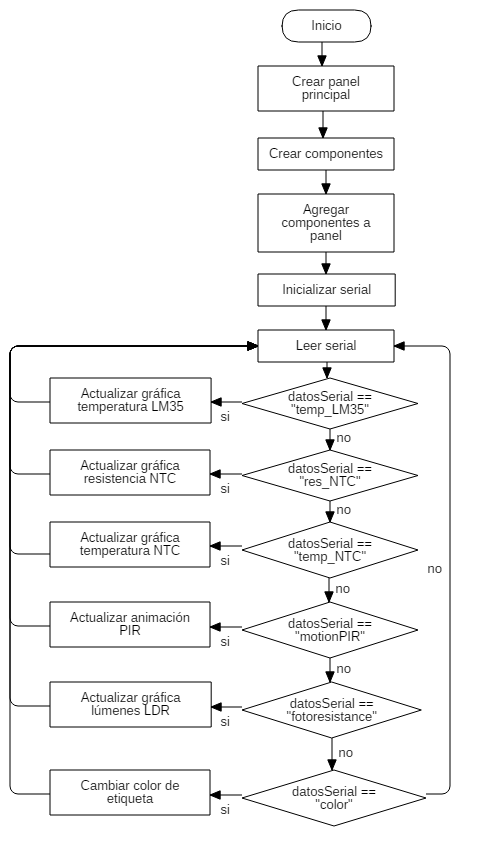
\includegraphics[width=\linewidth]{fig2_diagram_Hyperterminal.png}
  \caption{Diagrama de flujo de la programacion de la hyperterminal}
  \label{fig:flowDiagram2}
\end{figure}

La interfaz gráfica fue construida utilizando el lenguaje de programación Java y la implementación de la librería Java FX para el control de los gráficos.

Al iniciar el programa se obtienen los puertos disponibles, y se selecciona el puerto serial que se encuentra activo (por ejemplo, el COM1).

El proceso de graficación de los valores de los sensores se realiza a través de un hilo que corre constantemente mientras se ejecuta el programa. Continuamente se leen valores del búfer del microcontrolador que se imprimen a través del serial. 

Los valores que se reciben llegan en el siguiente formato “tipoDato,valorDato” como una cadena. Por ejemplo, en el caso del sensor de movimiento, la detección se recibe de la siguiente manera “motionSensor,0” o “motionSensor,1”.

Dicha cadena es dividida utilizando la coma como delimitador. La primera parte corresponde al tipo de valor recibido, que puede ser temperatura, resistencia, un valor de la memoria EEPROM o una tecla presionada. La segunda parte representa un valor que, dependiendo a que sensor corresponde, inicia un nuevo hilo que actualiza los valores de la gráfica, la repinta y finalmente elimina valores anteriores.

\section{Resultados}

\begin{figure}
  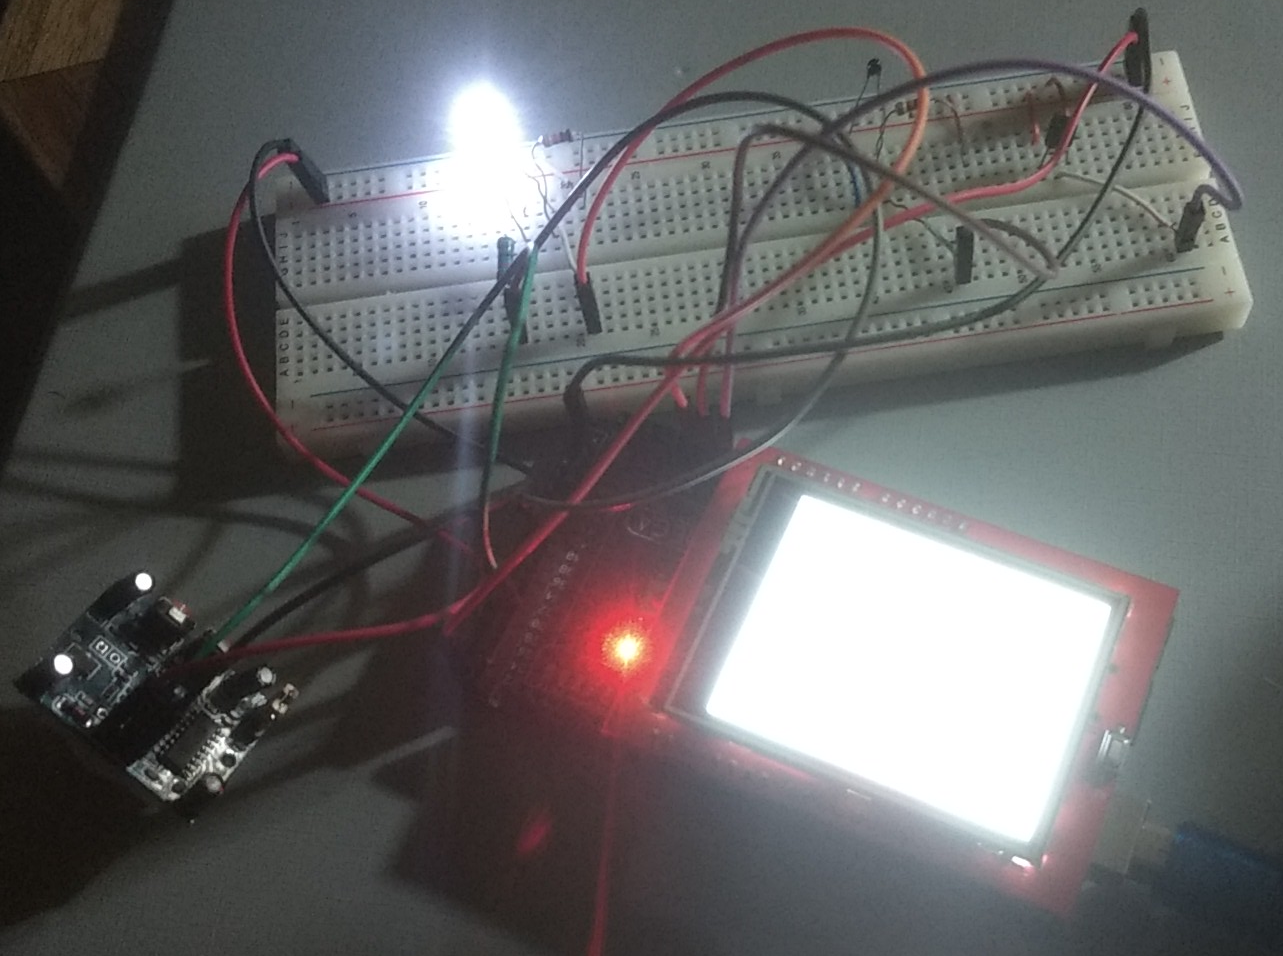
\includegraphics[width=\linewidth]{fig4_photo_Circuit.png}
  \caption{Fotografía del circuito armado}
  \label{fig:photo1}
\end{figure}

En la figura \ref{fig:photo1} se muestra el circuito armado terminado. En éste se incluyen el sensor de movimiento (PIR), una fotorresistencia (LDR), un sensor de temperatura (LM35) y un transistor (NTC), además de una pantalla TFT Shield y el mismo controlador Arduino Mega2560.

\begin{figure}
  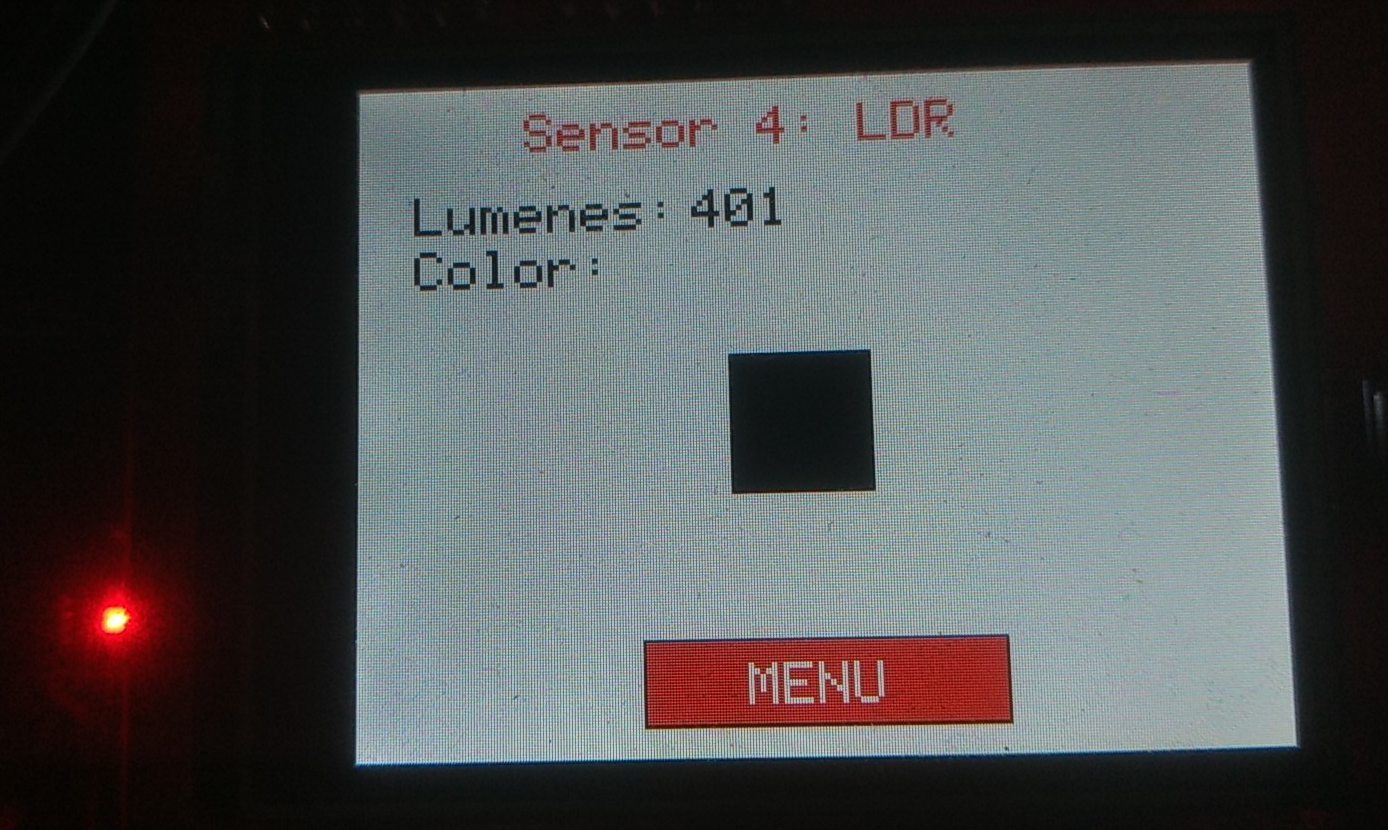
\includegraphics[width=\linewidth]{fig5_photo_Screen.png}
  \caption{Fotografía mostrando resultados de la fotorresistencia}
  \label{fig:photo2}
\end{figure}

En la figura \ref{fig:photo2} se puede apreciar la pantalla conectada al microcontrolador mostrando los valores obtenidos. En este caso, de la fotorresistencia se obtienen la cantidad de lúmenes y el color detectado.

\begin{figure}
  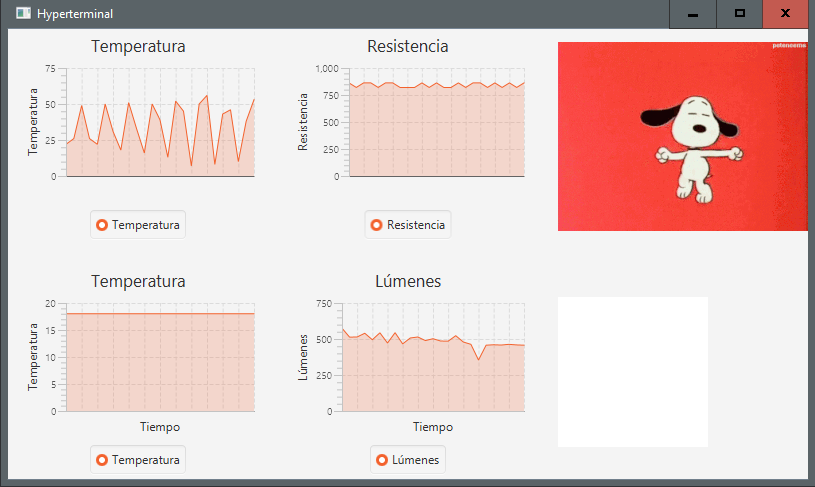
\includegraphics[width=\linewidth]{fig3_screenshot_Hyperterminal.png}
  \caption{Captura de pantalla de la hyperterminal}
  \label{fig:screenshot1}
\end{figure}

En la figura \ref{fig:screenshot1} se muestra la hyperterminal funcionando, leyendo valores enviados desde el microcontrolador a través del puerto serial y actualizando los diferentes componentes de la interfaz gráfica.

\section{Conclusiones}
Se tuvieron problemas en cuanto a la detección de lúmenes, debido a las variaciones que puede haber en el medio ambiente. 

Por parte de la programación del microcontrolador, se tuvieron problemas para realizar los menús y el teclado en la pantalla LCD, debido principalmente a que se deben pintar los componentes por separado y luego detectar las coordenadas en donde el usuario toca la pantalla. Para esto es necesario realizar la calibración de la misma detectando los valores máximos y mínimos en los ejes X y Y (horizontal y vertical) de la pantalla. La detección de las coordenadas debe ser constante, algo que no se había notado antes puesto que se estaban pintando los menús primero, y luego en base al menú en que se encuentran es la acción que se realiza.

También hubo conflicto al realizar la calibración de las variables de los sensores puesto que no se había contemplado en un inicio, lo que hizo necesario regresar al código terminado y modificar gran parte del mismo.

Otro problema que surgió es que existen diferentes librerías de código abierto que permiten la conexión serial entre Java y el microcontrolador, y desafortunadamente la escogida (RTXT) no permite la desconexión en caliente. Esto es, que mientras siga ejecutándose el programa, pueda ser posible desconectar el cable USB que va al Arduino y que, al realizar la reconexión, el programa continúe leyendo los valores. Esto ocurre ya que la librería bloquea por defecto el puerto serial al perder la conexión.

También se encontraron dificultades durante el desarrollo de la interfaz gráfica en Java. Ya que fue desarrollada utilizando Java FX, ésta tiene una manera diferente de crear e inicializar los componentes que la conforman. Una metáfora sería un escenario de una obra de teatro (el panel principal) compuesta por escenas más pequeñas (los componentes) que se añaden. A pesar de la dificultad inicial, Java FX facilita modificar el estilo gráfico de la interfaz utilizando hojas de estilo de cascada (CSS) como si se editara una página web HTML.

\section{Referencias bibliográficas}
\begin{thebibliography}{00}
\bibitem{b1} D., Hallee. "Passive Infrared Sensors: A Brief Overview". InHomeSafetyGuide.org. In Home Safety Guide. Retrieved 6 May 2016.
\bibitem{b2} Pallás Areny, R. (2007). Sensores y acondicionadores de señal. (4a. ed.). México D.F.: Alfaomega.
\bibitem{b3} Bastian, P. (2001). Electrotecnia (21a. ed.). México D.F.: Ediciones AKAL.
\bibitem{b4} Wayne, T. (2003). Sistemas de Comunicaciones Electrónicas. (4a. ed.). México D.F.: Prentice Hall.
\bibitem{b5} Arduino Mega 2560 R3 ~ Arduino.cl. (2014). Arduino.cl. Obtenido el 15 de noviembre de 2017, de http://arduino.cl/arduino-mega-2560/
\bibitem{b6} HyperTerminal. (2017). Technet.microsoft.com. Obtenido el 15 de noviembre de 2017, de https://technet.microsoft.com/en-us/library/bb490827.aspx
\bibitem{b7} 2.8" TFT Touch Shield v1 | Adafruit Shield Compatibility Guide | Adafruit Learning System. (2017). Learn.adafruit.com. Obtenido el 15 de noviembre de 2017, de https://learn.adafruit.com/adafruit-shield-compatibility/2-dot-8-tft-touch-shield
\bibitem{b8} Ramirez, E. V. (1986). En Limusa (Ed.), Introduccion a los microprocesadores: equipo y sistemas (1° ed., pag. 120). México D.F.
\end{thebibliography}

\end{document}
